% ---------------------------------------------------------------------------
% Author guideline and sample document for EG publication using LaTeX2e input
% D.Fellner, v1.13, Nov 13, 2007

\documentclass{egpubl}

% --- for  Annual CONFERENCE
\Seminar % Specialist Seminar (added by Ulrich Schwanecke (2019))
%\ConferenceSubmission % uncomment for Conference submission
%\ConferencePaper      % uncomment for (final) Conference Paper
%\STAR                 % uncomment for STAR contribution
% \Tutorial             % uncomment for Tutorial contribution
% \ShortPresentation    % uncomment for (final) Short Conference Presentation
%
% --- for  CGF Journal
% \JournalSubmission    % uncomment for submission to Computer Graphics Forum
% \JournalPaper         % uncomment for final version of Journal Paper
%
% --- for  CGF Journal: special issue
% \SpecialIssuePaper         % uncomment for final version of Journal Paper, special issue
%
% --- for  EG Workshop Proceedings
% \WsSubmission    % uncomment for submission to EG Workshop
% \WsPaper         % uncomment for final version of EG Workshop contribution
%
%\electronicVersion % can be used both for the printed and electronic version

% !! *please* don't change anything above
% !! unless you REALLY know what you are doing
% ------------------------------------------------------------------------

\PrintedOrElectronic

\usepackage[pdftex]{graphicx} 
\usepackage{t1enc, dfadobe}
\usepackage{egweblnk}
\usepackage{cite}

% For backwards compatibility to old LaTeX type font selection.
% Uncomment if your document adheres to LaTeX2e recommendations.
% \let\rm=\rmfamily    \let\sf=\sffamily    \let\tt=\ttfamily
% \let\it=\itshape     \let\sl=\slshape     \let\sc=\scshape
% \let\bf=\bfseries

% end of prologue

\usepackage{blindtext}
\usepackage{caption}
\usepackage{subfigure}
\usepackage{dblfloatfix}
\usepackage{adjustbox}
\usepackage{mathtools}
\usepackage{todonotes}
\usepackage{placeins}
\usepackage{listings, xcolor}
\usepackage[noabbrev]{cleveref}
\definecolor{ListingBackground}{HTML}{FCF7DE}

\lstset{
	language=bash,			% Standardsprache des Quellcodes
	% numbers=left,			% Zeilennummern links
	stepnumber=1,			% Jede Zeile nummerieren.
	numbersep=5pt,			% 5pt Abstand zum Quellcode
	numberstyle=\tiny,		% Zeichengrösse 'tiny' für die Nummern.
	breaklines=true,		% Zeilen umbrechen wenn notwendig.
	breakautoindent=true,	% Nach dem Zeilenumbruch Zeile einrücken.
	% postbreak=\space,		% Bei Leerzeichen umbrechen.
	postbreak=\mbox{\textcolor{red}{$\hookrightarrow$}\space},
	tabsize=2,				% Tabulatorgrösse 2
	basicstyle=\ttfamily\footnotesize, % Nichtproportionale Schrift, klein für den Quellcode
	showspaces=false,		% Leerzeichen nicht anzeigen.
	showstringspaces=false,	% Leerzeichen auch in Strings ('') nicht anzeigen.
	extendedchars=true,		% Alle Zeichen vom Latin1 Zeichensatz anzeigen.
	captionpos=b,			% sets the caption-position to bottom
	backgroundcolor=\color{ListingBackground}, % Hintergrundfarbe des Quellcodes setzen.
	xleftmargin=0pt,		% Rand links
	xrightmargin=0pt,		% Rand rechts
	frame=single,			% Rahmen an
	frameround=ffff,
	rulecolor=\color{darkgray},	% Rahmenfarbe
	fillcolor=\color{ListingBackground},
	keywordstyle=\color[rgb]{0.133,0.133,0.6},
	commentstyle=\color[rgb]{0.133,0.545,0.133},
	stringstyle=\color[rgb]{0.627,0.126,0.941},
	aboveskip=20pt,
}

% ---------------------------------------------------------------------
\captionsetup{labelfont=bf,textfont=it}
\title[]
      {Serverless Software License}

\author[B. Ahmad, J. Dujaka, E. Herwin, N. Sauer]
    {\parbox{\textwidth}
        {\centering 
			Bassir Ahmad, Janina Dujaka, Eduard Herwin, Niklas Sauer
        }
        \\
    {\parbox{\textwidth}
        {\centering RheinMain University of Applied Sciences, Wiesbaden, Germany\\
       }
    }
}
% ------------------------------------------------------------------------

% if the Editors-in-Chief have given you the data, you may uncomment
% the following five lines and insert it here
%
% \volume{36}   % the volume in which the issue will be published;
% \issue{1}     % the issue number of the publication
% \pStartPage{1}      % set starting page


%-------------------------------------------------------------------------
\begin{document}

%-------------------------------------------------------------------------
% uncomment for using teaser (comment if you don't want a teaser)
\teaser{
    \hspace{\fill}
    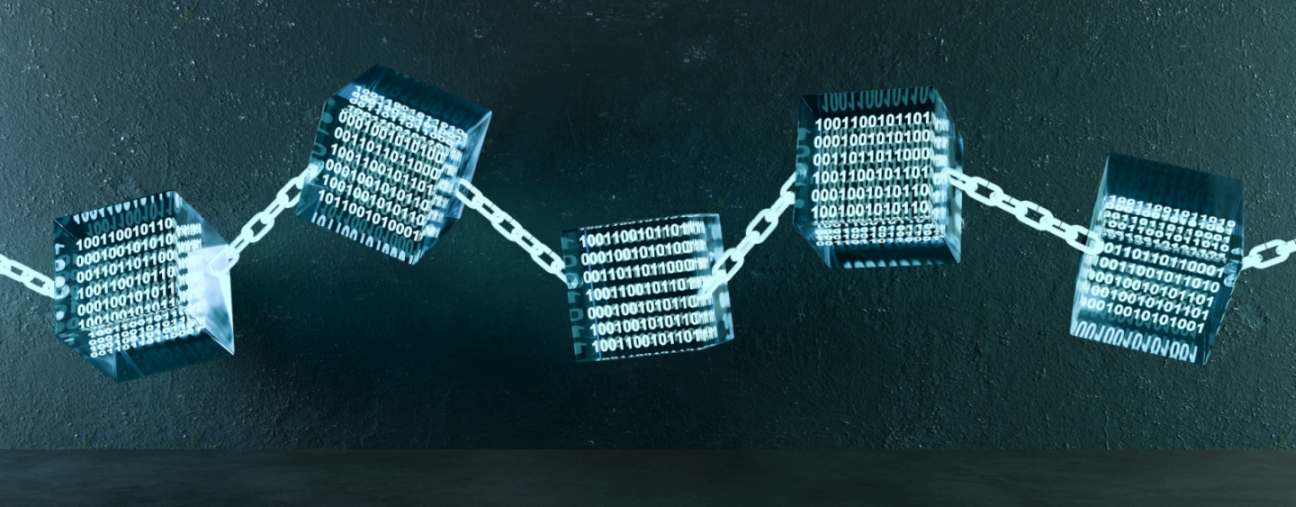
\includegraphics[width=1.0\linewidth]{images/header.jpg}\hfill
    \hspace{\fill}
    \centering
    % \caption{}
    %\label{fig:teaser}
}


%-------------------------------------------------------------------------
\maketitle


%-------------------------------------------------------------------------
% \begin{abstract}
% \end{abstract}  

%-------------------------------------------------------------------------

\section{Introduction}
\label{sec:introduction}
\begin{quote}
Licenses are boring. Blockchains in vogue, and on everyone's lips.
\end{quote}

This freely made up quote pretty much summarizes the attention both topics have received since Satoshi Nakamoto published his white paper on an electronic peer-to-peer network in 2008 \cite{nakamoto2019bitcoin}, shortly after which the first Bitcoins were mined, i.e. put into circulation. Both cryptocurrencies and the underlying blockchain technology have received much fanfare hereafter whereas licensing systems have practically remained the same. 

Usually, licensing involves a backend system that keeps records on valid activation codes as well as who purchased them initially. If the license is lost, support may be contacted but that leaves edge cases such as using an abandoned software application. Furthermore, this type of licensing does not allow for aftermarket reselling as any change of ownership would have to be communicated to the application developer. Both of these problems are tackled by the solution proposed in this paper.

The basic idea is to replace traditional database records with tokens on the blockchain. Combined with the public key cryptography inherent to such systems, license ownership claims can be autonomously verified. All without requiring applications developers to setup and maintain their own infrastructure.
 
To begin, essential concepts of blockchain technology are presented. Then the new blockchain way of licensing is explained in detail, followed by a short overview of the development and validation techniques used to create a reference implementation consisting of the token itself, a JavaScript client library as well as an Electron-based demo application. The paper concludes by summarizing the efforts and outlining potential future research topics.

%-------------------------------------------------------------------------

\section{Theoretical Framework}
In this section, we offer a brief guide on the mechanics of blockchains and usefulness of smart-contracts and tokens, both of which lead to the establishment of Ethereum, a second generation blockchain.  

\subsection{Blockchain}
A blockchain system is a special type of ledger that distributes its state across a large number of inter-connected nodes. Transactions describe modifications to this state. However, only those which are included in a block are considered to be effectual. To ensure that all nodes reach the same state, it is important that transactions are replayed in the same order. Therefore, each block of transactions is linked to the previous block, hereby creating a chronological chain of blocks - the blockchain. 

Various types of consensus algorithms have been developed to ensure that nodes agree on the actual ordering of blocks. In public permissionless blockchain systems, proof-of-work is currently the most prominent \cite{yim2018blockchain}.

\subsection{Wallets}
In its most narrow sense, a cryptocurrency wallet is a device, physical medium, program or service which stores public and/or private keys. From a user perspective, a public key allow others to make payments to that wallet, whereas a private key enables the spending of the funds received. The cryptocurrency itself is not stored in the wallet. Balances are recorded on the blockchain.

When designing wallets, comfort and privacy must be balanced. The simplest and most convenient wallet is one with a single private key and public address that can be reused multiple times. From a data protection perspective, this is not a good solution since everyone can easily track and correlate transactions through so-called block explorers. Using a new public address for each transaction is recommended but becomes very difficult to manage on one's own \cite{10.5555/2695500}.

\subsection{Smart-Contract}
In recent years, electronic contracts have regained the public's attention due to the rise of and embodiment in second generation blockchain technology. Smart-contracts are computer protocols that express and enforce a wide variety of contractual terms. For example, a bond based on a smart-contract could initiate interest payments to creditors on the interest date, or a corresponding insurance contract could automatically pay out the sum insured after an insurance claim has been verified. By automating manual tasks like these, considerable costs may be avoided \cite{smart-contract-definition}. 

\subsection{Tokens}
By introducing a digital equivalent, blockchain has evoked a semantic change for the word token originally used to mean privately-issued coin-like items that have insignificant value and are designed for a single purpose (e.g. transportation-, arcade- or laundry tokens). Now, tokens are used to simultaneously convey ownership, access rights, as well as the right to vote, for instance. Also, due to the blockchain's virtual nature, tokens become more easily exchangeable, a pitfall commonly cited \cite[p. 173]{10.5555/2695500}.

While some tokens represent blockchain-native digital items, many tokens are used to
represent extrinsic things. By such, one must keep in mind that human law or agreements oftentimes decide whether the transfer of ownership as expressed through tokens will be recognized \cite[p. 175-176]{10.5555/2695500}. 

\subsection{Ethereum}
Ethereum was designed to abstract the details of a blockchain to provide a deterministic and secure programming environment in which developers are no longer required to bootstrap the
underlying mechanisms \cite{10.5555/2695500}. It is practically regarded as an open-source, globally decentralized computing infrastructure that executes programs, known as smart-contracts, for which the current state and transitions leading to this state are stored in a blockchain alongside a cryptocurrency called Ether. It is primarily intended as a utility currency to meter and constrain resource usage during execution which stands in stark contrast with Bitcoin’s sole purpose of being a digital payment network \cite{10.5555/2695500}.

%-------------------------------------------------------------------------

\section{Design}
\label{sec:design}
In this section, the general idea for and design of a blockchain-based approach to software licensing is discussed. From a high-level perspective, the solution can be described as a combination of:

\begin{itemize}
   \item Tokens to track the licenses in circulation
   \item Public-key cryptography to verify the ownership of an address and thus the licenses associated with that address
\end{itemize}

\autoref{img:flowChart} shows the sequence of steps that will be necessary to either purchase a new, or activate an existing license. It preludes by assuming that a token exists (i) for each application wishing to utilize this blockchain way of licensing.

\begin{figure}[h]
	\centering
	\setlength{\fboxsep}{1pt}
   	\setlength{\fboxrule}{1pt}	
	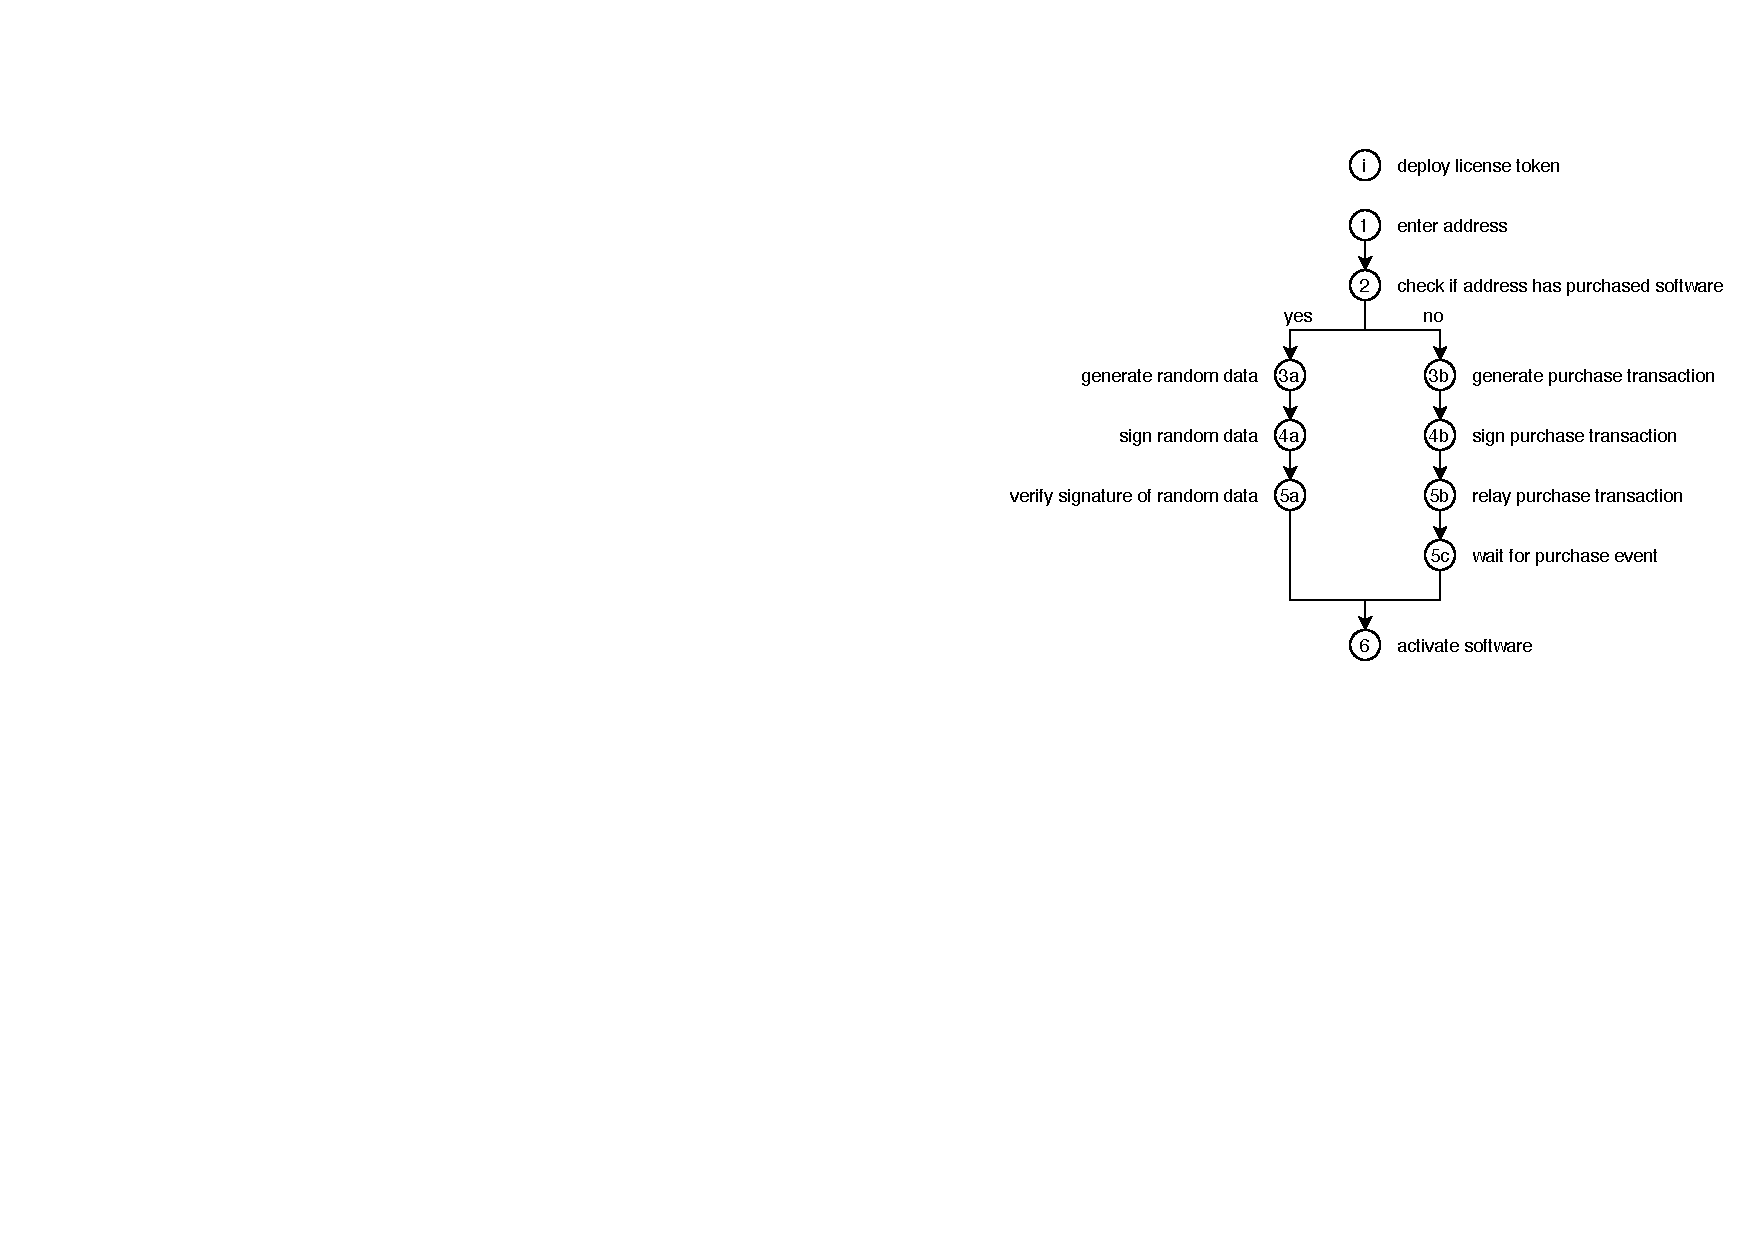
\includegraphics[width=1\linewidth]{images/flow_chart.pdf}
	\caption{License purchase and activation flow}
	\label{img:flowChart}
\end{figure}

\FloatBarrier

Naturally, the process will start by asking users to input their address (1) so that the system can check if a license is associated with that address or not (2). This leads to the following decision tree:

\begin{description}
	\item[Activate existing license \label{itm:activateFlow}]
	Because the solution assumes that a public permissionless blockchain will be used as the token's deployment target it is not sufficient to solely rely on the fact that an address owns a license token. Users could simply lookup the token's storage (\textit{registry}) to choose and input any of the addresses associated with a license. Therefore, the user is presented with an address ownership challenge leveraging the strengths of public key cryptography: it is easy to verify the signature of a message, i.e. figuring out the address used to generate that signature, but nearly impossible to produce a matching signature without possessing the private key. Consequently, the user is requested to sign (4a) randomly generated data (3a). Provided that the signature check passes (5a), the software may be activated (6).
	
	An important aspect of any licensing system is the ability to verify a previously activated license without recurrent user input. For security reasons, a boolean property list flag should not be considered, as attackers with file-level application access could set the activation state to their favor. Instead, a license file containing the address, challenge data and response is constructed and saved to some kind of storage, so that the same steps described beforehand may be conducted autonomously. However, a functioning internet connection is required to check whether the address still owns a license token. This aspect shall be determined by application developers. One may imagine that a certain grace period is given until a connection must be re-established. Similar solutions are found in products like Microsoft Office or Adobe Creative Cloud. 
	
	Taking a closer look at the mechanism provided to verify the license's status in the future by putting the address ownership challenge to storage, another potential security hole may come to mind in which attackers gain access to a plain text message and the corresponding signature generated by an address that luckily also owns a license token. These values could then be placed into storage to forge the activation scheme. To this end, a mitigation technique could be generating the random challenge data on-chain and resetting it for each and every license token transfer. It can be thought of as the equivalent to an activation code seen in traditional licensing systems but with the added requirement of having to sign it. This reduces the chances that a matching signature exists in the wild.
	\hfill \\
	\item[Purchase new license \label{itm:purchaseFlow}]
	Strictly speaking, this case can be seen as an extension to the upper. The difference being that a license token must first be purchased as the registry lookup would fail otherwise. And since transactions follow the same rules of public key cryptography, the signed and unsigned versions can be put to storage directly, foregoing the need to letting users sign randomly generated data. Unfortunately, this expedited activation method is incompatible with the additional security measure introduced above which necessitates that the signature must match that of an on-chain generated activation code. Again, the trade off between security and ease of use shall be decided by future application developers. 
	
	Another factor likely influencing this decision is the fact whether users shall be able to sign and relay the purchase transaction in-app or via their preferred channel. In the latter case, users would only get a pre-populated raw transaction (3b) that must be signed (4b) and relayed manually (5b). Afterwards, they are put into the \textit{\nameref{itm:activateFlow}} flow, thus re-requiring an address ownership challenge during which the stricter signature check can be applied. 
	
	Signing (4b) and relaying the purchase transaction in-app (5b) only makes sense if the user's private key can be securely injected into the application context. This doesn't actually require revealing the private key. External wallet providers and physical hardware devices such as the Ledger Nano S offer easy integration through their respective APIs. The return value is a signed transaction that may be relayed in-app and awaited upon by tracking its hash until included in a block (5c).
	\hfill \\
\end{description}

\autoref{img:appIntegration} attempts to map the steps of the newly devised licensing life-cycle to individual actors and components, giving an early look as to how the solution would be integrated with applications. It also emphasizes the fact that wallets do not have to be part of an application aiming to leverage a token-based licensing system. 

\begin{figure}[htbp]
	\centering
	\setlength{\fboxsep}{1pt}
   	\setlength{\fboxrule}{1pt}	
	
	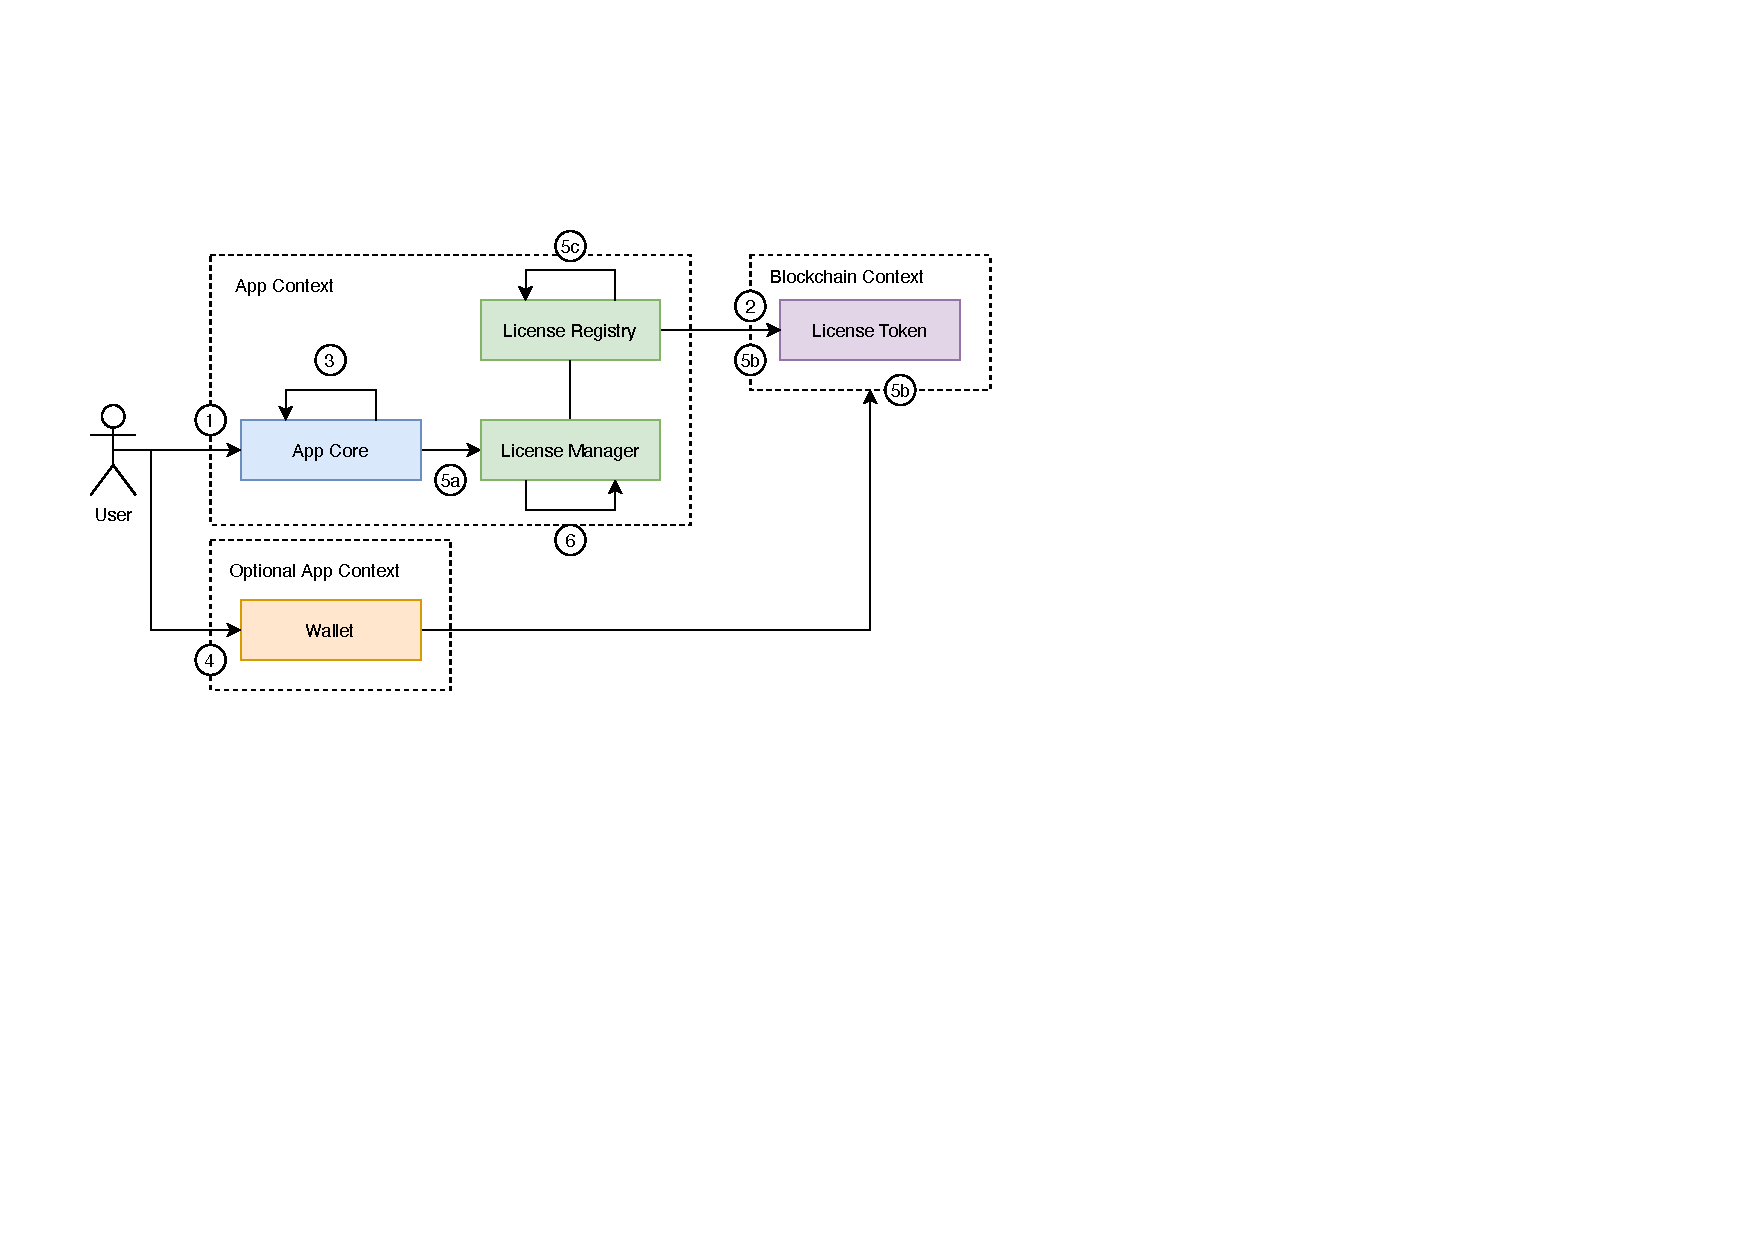
\includegraphics[width=1\linewidth]{images/app_integration.pdf}
	\caption{Integration with apps}
	\label{img:appIntegration}
\end{figure}

\FloatBarrier

%-------------------------------------------------------------------------

\section{Implementation}
The goal of this project is to provide application developers with a reference solution to running and interfacing with a token-based licensing system. As such, the main artifacts expected hereof are the token itself, as well as a client library handling the purchase and activation flows outlined in \autoref{sec:design}.

Most of today's decentralized application efforts target the web and are built upon technologies such as JavaScript (JS) \cite{goodman2007javascript}. It is therefore not a far stretch to first target this vast audience. However, JS and its weak typing system or the lack thereof make it hard to diagnose and catch bugs early. TypeScript (TS) on the other hand offers modern language features like static typing, generics and other syntactic sugar while still being fully compatible with standard JS runtimes \cite{bierman2014understanding}. This is achieved through so-called transpilers that convert code to equivalent statements of such.

Given the repeatedly expressed requirement of utilizing tokens to convey ownership of and usage rights to software, it becomes clear that first generation blockchains like Bitcoin do not suit this use case. Instead, Ethereum and its various token standards (e.g. ERC-20 or ERC-721) have been chosen for this project which is also largely due to its rich and highly maintained ecosystem of developer tools such as Ganache \cite{lee2019testing}. Ganache is a personal blockchain for rapid Ethereum and Corda distributed application development \cite{brown2016corda}. Together with Truffle, a testing framework, Ganache can be used during the entire development cycle, offering a safe and deterministic environment to develop, deploy and test applications. Nevertheless, it is good practice to also test the application against one of Ethereum's public testnets which more accurately resemble production behaviour. \Cref{lst:startGeth,lst:unlockAccount,lst:deployContract} demonstrate the deployment process to Ethereum's Goerli testnet which is based on proof-of-authority.

Generally, the implementation followed a top-down approach, meaning that the requirements expressed by \autoref{img:flowChart} were first mapped onto individual components (\autoref{img:appIntegration}), then organized into and specified as classes (\autoref{img:classDiagram}) and lastly translated to suitable TS interfaces. This work breakdown structure could then be assigned for development.

%-------------------------------------------------------------------------

\section{Validation}

A rigid suite of unit tests hopes to ensure the implementation's correctness. Unit testing is a software testing method by which individual units of source code, sets of one or more computer program modules together with associated control data, usage and operating procedures, are tested to determine whether they are fit for use. Test-driven development helps programmers clarify what a code segment is actually supposed to do by requiring the accompanying tests to be written beforehand. Combined with an automated testing environment, this leads to the following benefits:

\begin{itemize}
   \item Tests showcase which segments have actually been executed (coverage)
   \item Tests can be rerun to ensure that changes have not introduced new bugs (regression)
   \item Tests pinpoint the root causes of problems (debugging)
   \item Tests describe what the code should do (documentation)
\end{itemize}

Given the scale of the project, it has been decided to mainly rely on requirements-based testing, which is a semantic approach to test-case design where a set of tests is derived for each requirement.

To further demonstrate the design's effectiveness, another small application was created acting as the end-to-end test bed. This demo app is also useful for giving other developers a sense as to how the JS client library produced here may be integrated with their applications, especially those based on the React UI framework. It was built using Electron (formerly Atom Shell) which is an open-source framework developed by GitHub that enables the development of cross-platform desktop applications using the Chromium web browser and Node.js runtime \cite{electron}. Electron was developed as the basis for GitHub's Atom editor, and is also the foundation for Visual Studio Code. \autoref{img:demoAppScreenshots} is a collection of app screenshots in which the points 1.1 to 1.4 show how the purchase of a new license works. Points 2.1 to 2.3 deal with restoring a previously purchased license.

%-------------------------------------------------------------------------

\section{Conclusion}
This paper highlighted the problems of current licensing systems, laid out the fundamentals of blockchain technology and used two of its key strengths to propose a new token-based approach. This approach replaces traditional database records with tokens and validates an ownership claim by employing a simple but effective public key cryptography challenge.

As a proof-of-concept, both a \href{https://github.com/niksauer/serverless-software-license}{token and JS client library} have been developed. They are fully documented, tested and published to the \href{https://www.npmjs.com/package/serverless-software-license}{Node Package Manager}. Further, an \href{https://github.com/niksauer/serverless-software-license-example}{Electron demo application} has been created utilizing the aforementioned library. Both efforts should help interested parties in understanding how the individual components work in conjunction. 

The project also opens the possibility for creating an after-sale license marketplace. Another aspect that might be of future research interest is the choice of token standard employed. Here, the simple ERC-20 interface has been chosen but alternatives like ERC-721 would allow for attributing individual licenses. An obvious use case for this is differentiating between individual and family licenses.

In total, the authors have identified yet another business area for blockchain technology - the blockchain way of licensing. 

%-------------------------------------------------------------------------

%\bibliographystyle{eg-alpha}
\bibliographystyle{eg-alpha-doi}
\bibliography{bibliography}

%-------------------------------------------------------------------------
% Appendix

\begin{figure*}[h]
	\centering
	\setlength{\fboxsep}{1pt}
   	\setlength{\fboxrule}{1pt}	
	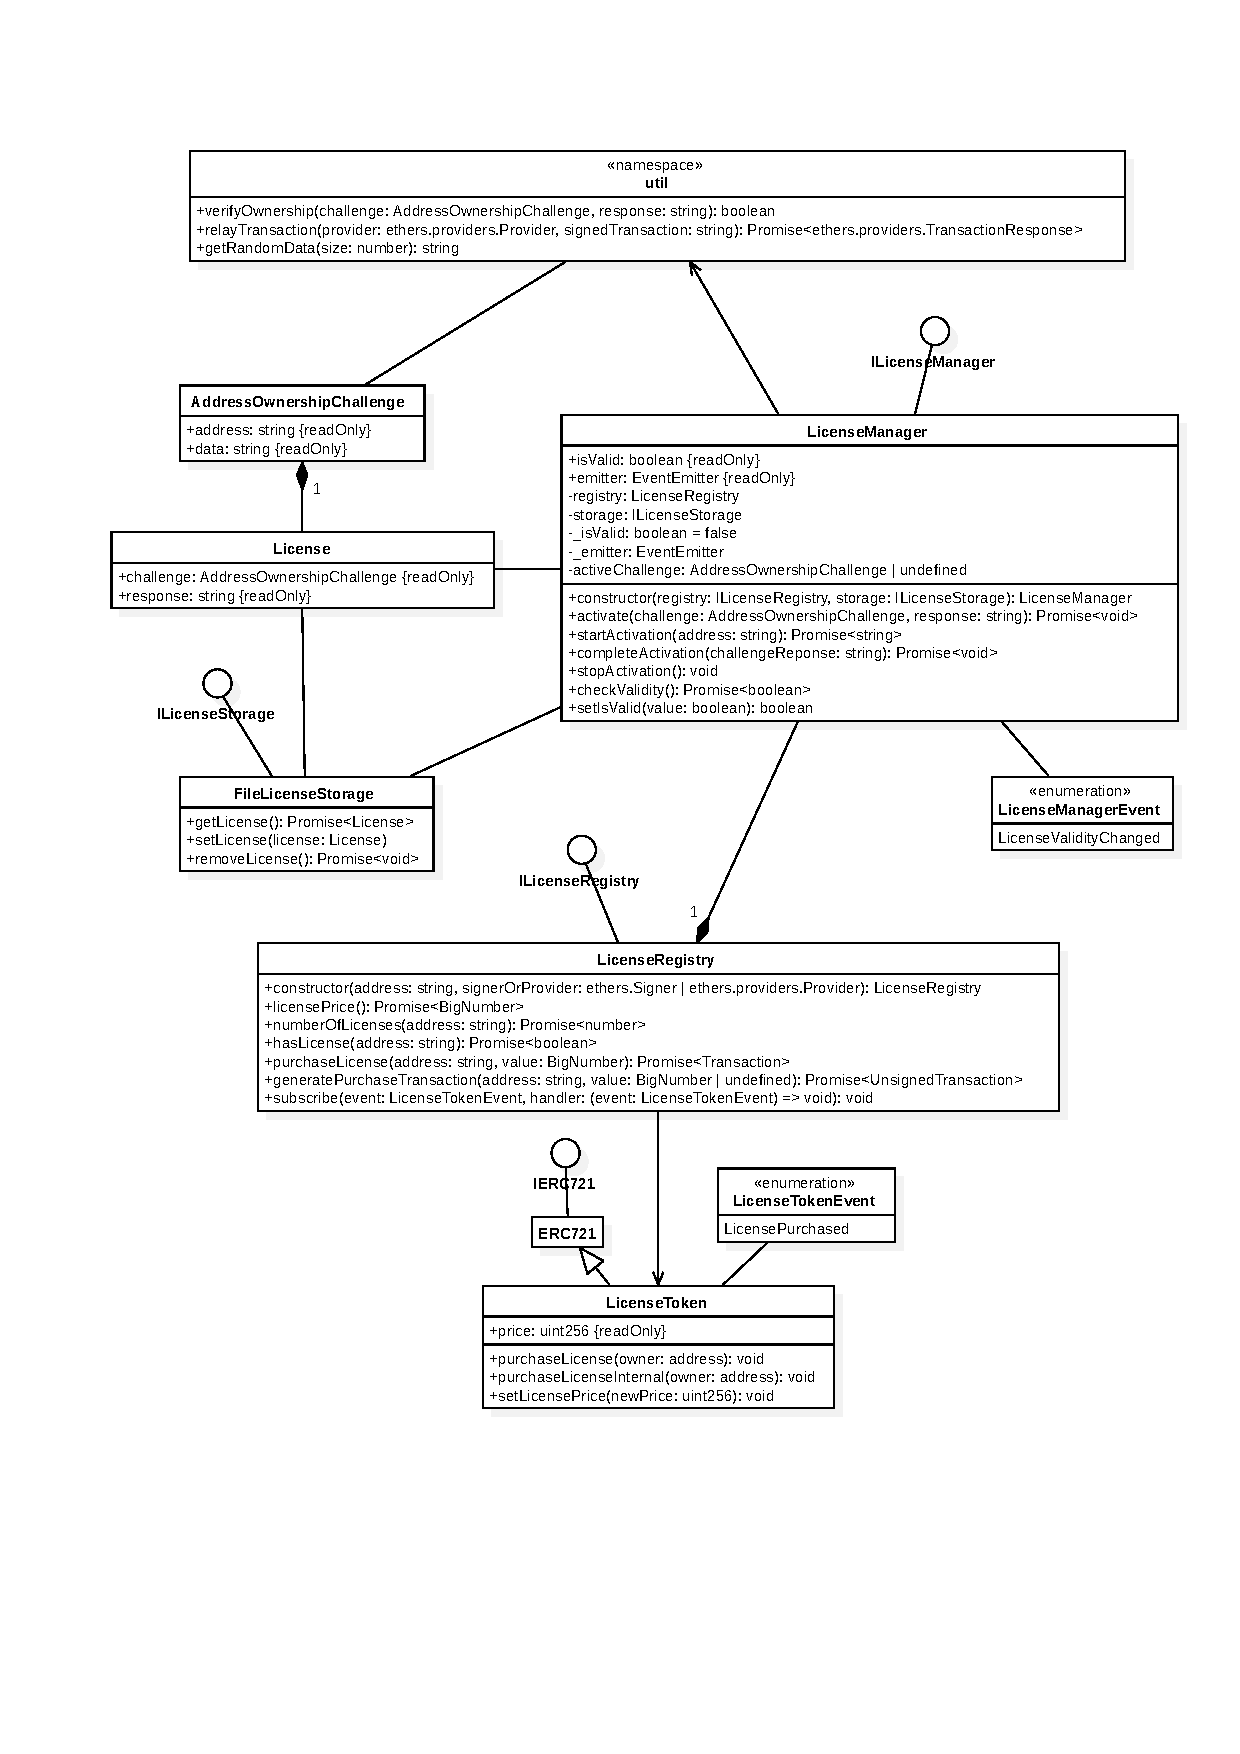
\includegraphics[width=1\linewidth]{images/class-diagram.pdf}
	\caption{Client library class diagram}
	\label{img:classDiagram}
\end{figure*}

\FloatBarrier

\begin{lstlisting}[language=bash, caption=Start Geth testnet client and create new account, label=lst:startGeth]
$ git clone git@github.com:niksauer/blockchain-lab.git
$ cd blockchain-lab
$ docker-compose -f docker-compose-geth.yml up

$ docker-compose -f docker-compose-geth.yml exec geth /bin/sh
$ > geth account new --datadir /root/.ethereum/goerli/

Your new account is locked with a password. Please give a password. Do not forget this password.
Password: <password>
Repeat password: <password>

Your new key was generated

Public address of the key:   0x0cBA519aC95879BDE88C975E918F78270972AF30
Path of the secret key file: /root/.ethereum/goerli/keystore/UTC--[...]

$ > geth account list --datadir /root/.ethereum/goerli

Account #0: {0cba519ac95879bde88c975e918f78270972af30} keystore:///root/.ethereum/goerli/keystore/UTC--[...]
\end{lstlisting}

\begin{lstlisting}[language=bash, caption=Unlock account for JSON-RPC usage, label=lst:unlockAccount]
$ docker-compose -f docker-compose-geth.yml exec geth /bin/sh
$ > geth attach --datadir /root/.ethereum/goerli/
$ >> web3.personal.unlockAccount("0x0cBA519aC95879BDE88C975E918F78270972AF30")

Unlock account 0x0cBA519aC95879BDE88C975E918F78270972AF30
Passphrase: <password>
true
\end{lstlisting}

\begin{lstlisting}[language=bash, caption=Deploy smart-contract, label=lst:deployContract]
$ git clone git@github.com:niksauer/serverless-software-license.git
$ cd serverless-software-license/ethereum
$ truffle migrate --network goerli

Compiling your contracts...
===========================
> Everything is up to date, there is nothing to compile.



Migrations dry-run (simulation)
===============================
> Network name:    'goerli-fork'
> Network id:      5
> Block gas limit: 8000000 (0x7a1200)


1_initial_migration.js
======================

   Deploying 'Migrations'
   ----------------------
   > block number:        3010942
   > block timestamp:     1594220218
   > account:             0x0cBA519aC95879BDE88 C975E918F78270972AF30
   > balance:             0.399701218
   > gas used:            149391 (0x2478f)
   > gas price:           2 gwei
   > value sent:          0 ETH
   > total cost:          0.000298782 ETH

   -------------------------------------
   > Total cost:         0.000298782 ETH


2_deploy_contracts.js
=====================

   Deploying 'LicenseToken'
   ------------------------
   > block number:        3010944
   > block timestamp:     1594220219
   > account:             0x0cBA519aC95879BDE88 C975E918F78270972AF30
   > balance:             0.396531474
   > gas used:            1557531 (0x17c41b)
   > gas price:           2 gwei
   > value sent:          0 ETH
   > total cost:          0.003115062 ETH

   -------------------------------------
   > Total cost:         0.003115062 ETH


Summary
=======
> Total deployments:   2
> Final cost:          0.003413844 ETH





Starting migrations...
======================
> Network name:    'goerli'
> Network id:      5
> Block gas limit: 8000000 (0x7a1200)


1_initial_migration.js
======================

   Deploying 'Migrations'
   ----------------------
   > transaction hash:    0xbe1782bafa9851d7efd4 7962c8b0d1d856ed008241f1a97ee738ad f5c55aa138
   > Blocks: 0            Seconds: 12
   > contract address:    0x1C87AbeB6da182db792f f091d712760c60c1bB93
   > block number:        3010942
   > block timestamp:     1594220234
   > account:             0x0cBA519aC95879BDE88C 975E918F78270972AF30
   > balance:             0.39671218
   > gas used:            164391 (0x28227)
   > gas price:           20 gwei
   > value sent:          0 ETH
   > total cost:          0.00328782 ETH


   > Saving migration to chain.
   > Saving artifacts
   -------------------------------------
   > Total cost:          0.00328782 ETH


2_deploy_contracts.js
=====================

   Deploying 'LicenseToken'
   ------------------------
   > transaction hash:    0xba6f7b47e6c0005e45cd e171d0fb229d1451bc20114cdf7e1eaf87c aa650e86f
   > Blocks: 0            Seconds: 12
   > contract address:    0x9CcB19007Fa23CbEB7c 74A62CD7aaBD255C183ab
   > block number:        3010945
   > block timestamp:     1594220279
   > account:             0x0cBA519aC95879BDE88 C975E918F78270972AF30
   > balance:             0.36321474
   > gas used:            1632531 (0x18e913)
   > gas price:           20 gwei
   > value sent:          0 ETH
   > total cost:          0.03265062 ETH


   > Saving migration to chain.
   > Saving artifacts
   -------------------------------------
   > Total cost:          0.03265062 ETH


Summary
=======
> Total deployments:   2
> Final cost:          0.03593844 ETH
\end{lstlisting}


\FloatBarrier

\begin{figure*}[h]
	\centering
	\setlength{\fboxsep}{1pt}
   	\setlength{\fboxrule}{1pt}	
	\includegraphics[width=1\linewidth]{screenshots/all_screenshots.png}
	\caption{Demo application with license purchase and activation flow}
	\label{img:demoAppScreenshots}
\end{figure*}

\end{document}